\chapter{Concept of Spark based Semantic Document Matching}
\label{concept}

In this Chapter, We discuss the motivation involved in the design and implementation of the document matching application using Apache Spark. In \ref{section: Idea}, we discuss the idea of our application. In \ref{section: workflow of spark based document matching}, We discuss the stages involved in implementation procedure of Document matching application.

\section{Overview}
\label{section: Idea}
As discussed earlier in \ref{background}, matching the similarity between two documents based on their semantics using TF-IDF model is not reliable. The TF-IDF techniques are mostly dependent on word occurrences in any document. But, Latent Dirichlet Allocation (LDA) represents any given document in terms of topic distribution by discovering the latent topics as discussed in \ref{section: lda}. 

\par The latent topics found by LDA translates to the contextual representation of a document. The context of the document speaks about how a document is structured. If we have the structure of the documents in terms of topic distribution then why should not the documents be compared?  This question has motivated us to design and implement the document matching application using LDA technique.

\par On the other side, we aimed to process the huge collection of documents. In recent times, MapReduce has been widely used programming model. But MapReduce has some performance limitations when compared to Apache Spark primarily in the area of iterative algorithms and are discussed in \ref{section: Mapreduce}. Since our motivation also includes in reducing the execution time of the application, we have used the Apache Spark as our parallel processing framework. The processing of in-memory computations, support for iterative algorithms are some of the advantages of Apache Spark and additional information is available in \ref{section: apache spark}.

\par Our objective was to increase the efficiency of our application and also present the potential of the Apache Spark framework. We did not made any modifications or improvements to the LDA algorithm but focused on finding a way to reduce the execution time.

\section{Workflow of Spark based Document Matching}
\label{section: workflow of spark based document matching}

As we have discussed our idea behind document matching using LDA. We now discuss the working model of our document matching application. The implementation of our application consists of 8 stages starting from loading of data to evaluation stage. The working process of our application using Apache Spark components is illustrated in \ref{fig: Implementation_process}.
\begin{figure}[htbp]
	\centering
		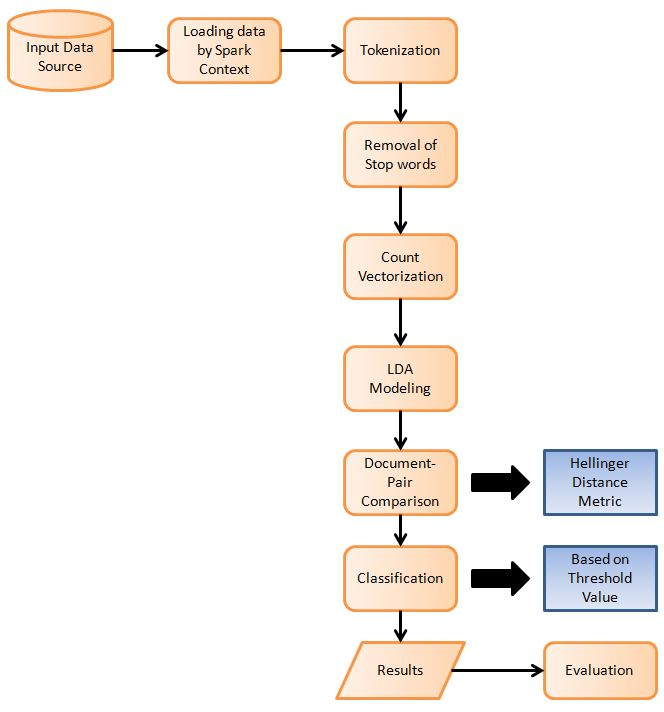
\includegraphics[scale=0.90]{implementation_process}
	\caption{Implementation procedure for Document Matching Application}
	\label{fig: Implementation_process}
\end{figure}

\newpage
\par From \ref{fig: Implementation_process}, the initial stage of our implementation starts by loading data from the external sources. It is a corpus in our case. The data will be loaded as a DataFrame with the help of Spark SQL.Each row of the DataFrame represents one document. The data in DataFrame is then sent as input to the tokenizer which extracts features from the document. In Stop words removal stage, further cleaning of the data such as removal of English stop words that do not contribute to the term importance is performed on the output of the tokenizer stage. In Count Vectorizer stage, every unique term is mapped to a unique ID and converts the documents to a sparse vectors representation. It is now time for topic modeling using LDA technique in LDA modeling stage. The total documents are compared with each other and an additional column containing match score is added to the DataFrame in the Document Pair Comparison Stage. Using the predefined threshold value, the document pairs are classified as matches and non-matches in the classification stage. The document pairs classified are then stored as a DataFrame. In the evaluation stage, the classified pairs are evaluated as true positives, false positives, true negatives and false negatives. 

\par Using Apache Spark framework, it is possible to execute each stage of our application individually by storing each stage result and then feeding as input to the future stage. Alternatively, all the stages can be executed as a chain of processes without writing intermediate results to the disk. The requirements, the details of our Spark based Document Matching implementation and the transformations of data at every stage are discussed in \ref{implementation}.


